\documentclass[./main.tex]{subfiles}

\begin{document}
\chapter{Analisi Sperimentale}
% ------------- La libreria TPTP -------------
\section{La libreria TPTP}
\begin{figure}[h]
    \centering
    \scalebox{0.3}{
        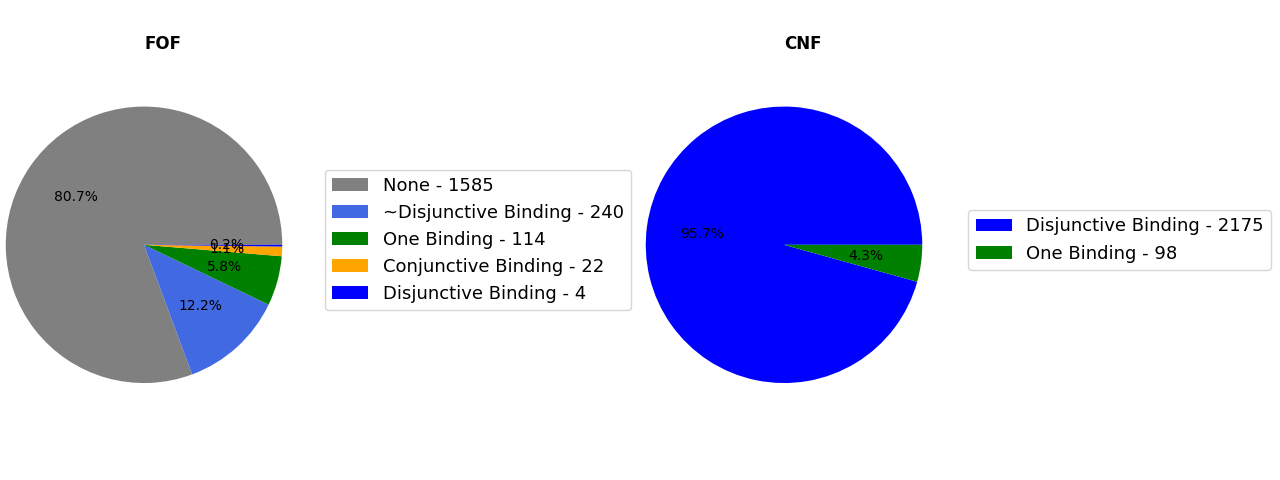
\includegraphics{images/5_sperimentazione/fof_cnf_classificazione.png}
    }
    \caption{Classificazione Libreria TPTP fof e cnf senza uguaglianza}
    \label{fig:classificazione_tptp}
\end{figure}

Per verificare la correttezza e l'efficienza dell'algoritmo implementato è stata scelta 
la libreria di problemi TPTP \cite{tptpLib} come dataset di problemi da risolvere. 
La libreria TPTP è una collezione di problemi per sistemi ATP dove ogni problema è scritto in formato
TPTP come descritto nella sezione \ref{sec:tptp_lang}.
I problemi TPTP sono suddivisi in base al dominio di appartenenza e il formato (fof, cnf, tff, ecc).
Il nome dei file segue il seguente schema:
\begin{verbatim}
    <domain><number>[+,-]{.<variant>}.p
\end{verbatim}

dove '$<$domain$>$' è il dominio di appartenenza del problema composto da tre lettere maiuscole e
'$<$number$>$' è un numero, generalmente di tre cifre che identifica il problema all'interno del dominio.
Il simbolo + indica che il problema è scritto con la sintassi \textit{fof} mentre il simbolo - indica
che il problema è scritto con la sintassi \textit{cnf}. '.$<$variant$>$' è un suffisso opzionale che
identifica una variante del problema ed in generale è un numero a tre cifre.
Ad esempio un nome valido è \textit{SYN001+1.003.p} che indica il problema 1 del dominio \textit{Syntactic},
in formato \textit{fof}, variante 3. 

Non tutti i problemi sono adatti per essere risolti con l'algoritmo implementato ed è 
stato quindi necessario filtrare i problemi in base a determinate caratteristiche.
In primo luogo sono stati scartati tutti i problemi non in formato \textit{fof} o \textit{cnf} e
i problemi con uguaglianza. Questo è stato possibile tramite il comando \textit{TPTP2T}:

\begin{itemize}
    \item Per i problemi fof: \texttt{tptp2T -q2 -pps Form FOF -Equality}
    \item Per i problemi cnf: \texttt{tptp2T -q2 -pps Form CNF -Equality}
\end{itemize}

Il risultato delle due query ha restituito una lista di \textbf{1969} problemi in formato \textit{fof} e
\textbf{2274} problemi in formato \textit{cnf}. 
Da entrambe le liste è stato scartato un problema puramente proposizionale,
quindi poco significativo per la sperimentazione, ma estremamente grande da rallentare l'intero set di benchmark,
riducendo il numero di potenziali problemi utili a \textbf{1965} per i problemi \textit{fof} e \textbf{2273} per i problemi \textit{cnf}.

Successivamente tutti i problemi sono stati classificati tramite il classificatore descritto nella sezione \ref{sec:classifier}.
Si ricorda che i problemi sono dati in formato $(A_1 \land A_2 \land ... \land A_n) \Rightarrow C$ dove 
$A_1, A_2, ..., A_n$ sono assiomi e $C$ è la congettura, mentre 
sia l'algoritmo di decisione che Vampire lavorano sul problema negato ovvero $A_1 \land A_2 \land ... \land A_n \land \lnot C$.
Per classificazione di un problema $P$ con congettura si intende quindi il frammento di appartenenza del problema negato $\lnot P$.
Nelle formule in cui non è presente la congettura, come quelle del formato \textit{cnf}, per classificazione della formula $P$ si intende il frammento di appartenenza del
problema non negato $P = A_1 \land ... \land A_n$.
I risultati della classificazione sono mostrati in figura \ref{fig:classificazione_tptp}.

Riguardo i problemi \textit{fof}, dei 1965 problemi analizzati:
\begin{itemize}
    \item \textbf{1585} sono stati classificati come \textit{None} e quindi totalmente inutilizzabili.
    \item \textbf{114} sono \textit{One Binding} e \textbf{22} sono \textit{Conjunctive Binding}, quindi adatti per l'algoritmo.
    \item \textbf{244} sono \textit{Disjunctive Binding} e quindi non adatti per l'algoritmo.
\end{itemize}
Dei 244 problemi \textit{Disjunctive Binding}: \textbf{240} contengono la congettura mentre gli altri \textbf{4} non la contengono.
I 240 problemi con la congettura sono stati recuperati negandoli in modo tale da portarli nel formato $\lnot A_1 \lor ... \lor \lnot A_n \lor C$ 
che fa parte del frammento \textit{Conjunctive Binding} e quindi adatto per l'algoritmo 
(questi problemi nella figura \ref{fig:classificazione_tptp} sono chiamati \textit{$\sim$Disjunctive Binding}).
Questo porta ad un numero totale di \textbf{376} problemi utili in formato \textit{fof}.

Riguardo i problemi \textit{cnf}, la suddivisione è più netta.
Tutte le formule CNF sono infatti o del frammento \textit{One Binding}, se per ogni clausola
tutti i letterali della clausola hanno la stessa lista di termini, o altrimenti del frammento \textit{Disjunctive Binding}.
Dei 2273 problemi analizzati:
\begin{itemize}
    \item \textbf{98} sono del frammento \textit{One Binding}
    \item \textbf{2175} sono del frammento \textit{Disjunctive Binding}
\end{itemize}
In questo caso la negazione delle formule \textit{Disjunctive Binding} porterebbe a problemi puramente proposizionali e quindi poco utili per la sperimentazione.
Il totale dei problemi utili in formato \textit{cnf} è quindi di \textbf{98}. Per un totale di \textbf{474} problemi utili.
La lista dei 474 problemi è riportata nell'appendice \ref{app:numerazione_problemi}.
Ogni problema è stato numerato nella tabella \ref{tab:numerazione_problemi} per essere facilmente identificato.
% ------------- La libreria TPTP -------------


% ------------- Analisi dei risultati -------------
\section{Analisi dei risultati}
In questa sezione verranno analizzati i risultati dell'esecuzione dell'algoritmo sui problemi selezionati nel paragrafo precedente
e confrontati con i risultati ottenuti da Vampire. 
L'obbiettivo della sperimentazione è confrontare l'efficienza di un algoritmo gneral purpose basato su Resolution come quello implementato da Vampire
con un algoritmo specializzato SMT come quello implementato.
Vampire implementa numerose strategie, euristiche e inferenze di semplificazione per essere efficiente a livello competitivo
quindi per indurlo a comportarsi il più possibile come il modello della \textit{Given Clause} descritta 
nella sezione \ref{sec:vampire_saturazione} è stato necessario disabilitare/impostare alcune opzioni.
In particolare sono state disattivate tutte le semplificazioni 
e le euristiche applicabili ad entrambi gli approcci ma non presenti in modo comune alle attuali implementazioni.
L'algoritmo di saturazione adottato è stato \textit{Otter}, 
poiché l'algoritmo predefinito \textit{LRS} non offre garanzie di completezza e
si basa sull'uso di limiti di tempo e memoria come criteri di selezione/semplificazione. 
È preferibile evitare questa metodologia poiché si desidera che gli algoritmi confrontati abbiano quantomeno lo stesso input.
Anche per il preprocessing sono state disabilitate tutte le semplificazioni non comuni a entrambi gli algoritmi.
In particolare l'opzione \textit{-updr} (Unused Predicate Definition Removal) è stata disabilitata in quanto non utilizzata dall'algoritmo
Binding. 
Come regola di semplificazione è stata disattivata l'opzione \textit{-fs} (Forward Subsumption) che elimina 
clausole che sono sussunte da altre clausole durante la fase di \textit{Forward simplification} 
(Una clausola $D$ è sussunta da una clausola $C$ se esiste una sostituzione $\sigma$ tale che 
$C^\sigma \subseteq D$, clausole del genere vengono cercate dalla $fs$ e rimosse perchè ridondanti).
È stata disattivata anche l'opzione \textit{-av} (AVATAR-Advanced Vampire Architecture
for Theories and Resolution) che è un metodo SMT implementato in Vampire per lo splitting delle clausole.
L'opzione \textit{-av} è stata disattivata dato che non si vuole che Vampire utilizzi metodi SMT per la risoluzione dei problemi.
Il comando utilizzato per l'esecuzione di Vampire è quindi il seguente:
\begin{verbatim}
    vampire --mode vampire -sa otter -t 10m -m 12000 -av off -updr off -fs off <problem>
\end{verbatim}
Dove \textit{$<$problem$>$} è il problema da risolvere. 
Come limiti di tempo e memoria sono stati impostati rispettivamente 10 minuti e 12GB di ram.
L'algoritmo Binding è stato eseguito con i seguenti parametri:
\begin{verbatim}
    vampire --mode 1b -t 10m -m 12000 <problem>
\end{verbatim}
I seguenti risultati sono estrapolati dall'esecuzione del programma su un 
Macbook Pro 2018, 2.9 GHz 6-Core Intel Core i9, 16 GB 2400 MHz DDR4 sistema operativo macOS Sonoma 14.0.
Gli esperimenti sono stati poi ripetuti su un computer Windows 11 con processore Intel Core i9-13900K e ram 32GB DDR5
sul sottosistema Windows for Linux (WSL) e si sono ottenuti tempi di esecuzione, come da aspettativa, più bassi ma assolutamente coerenti,
mentre per memoria i valori sono rimasti esattamente gli stessi.


\section{Ottimizzazioni}
\section{Conclusioni e Possibili Sviluppi futuri}

\end{document}